%!TeX root=../tese.tex
%("dica" para o editor de texto: este arquivo é parte de um documento maior)
% para saber mais: https://tex.stackexchange.com/q/78101


\chapter{NLP Techniques}
In this chapter we intend to present an overview of some of the NLP concepts, mostly based on neural networks, which are relevant to comprehend this project. As previously mentioned, we intend to leverage NLP techniques to perform the code processing technique of automating function extractions. While some methods can be used as is, others can barely be used at all. In further chapters their usage and limits for our use case will be further explored, while in this chapter they are only going to be introduced to the readers to better situate them.

\section{Embeddings}

When we are dealing with neural networks, we are essentially dealing with matrix operations, so in order to apply NNs to NLP tasks one first needs to somehow transform words and sentences into numbers.


A rudimentary approach would be an one-hot-encoding, where given a vocabulary of size $V$ we have a vector of size $V$ with each word of the vocabulary being associated to a specific index of our vector in a one-to-one fashion, where it is 0 at every index except for the one corresponding to the word to be represented. Fig.~\ref{fig:poke} illustrates, with categorical variables, the one-hot-encoding. Another similar concept is called bag of words, a sentence representation obtained by adding the one-hot-encoding of the words in said sentence.


\begin{figure}
\centering
\begin{subfigure}{.5\textwidth}
  \centering
  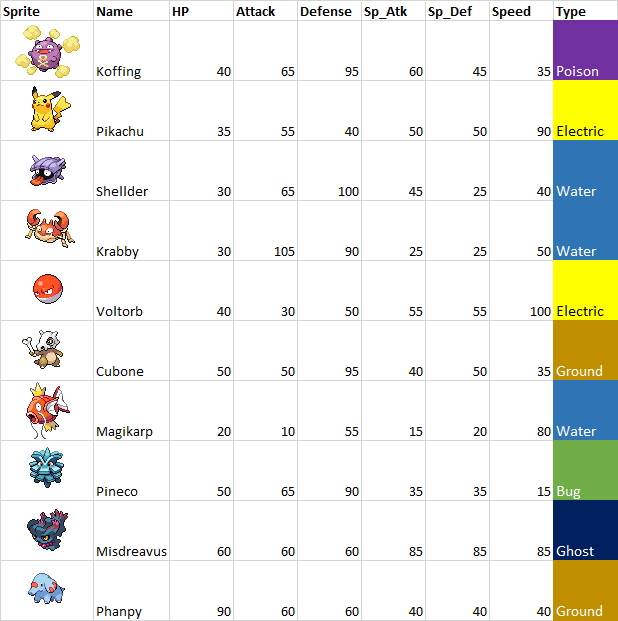
\includegraphics[width=1\linewidth]{figuras/pokemon_cate.png}
  \caption{Categorical representation of Pokémon types.}
  \label{fig:pokecat}
\end{subfigure}
\begin{subfigure}{.7\textwidth}
  \centering
  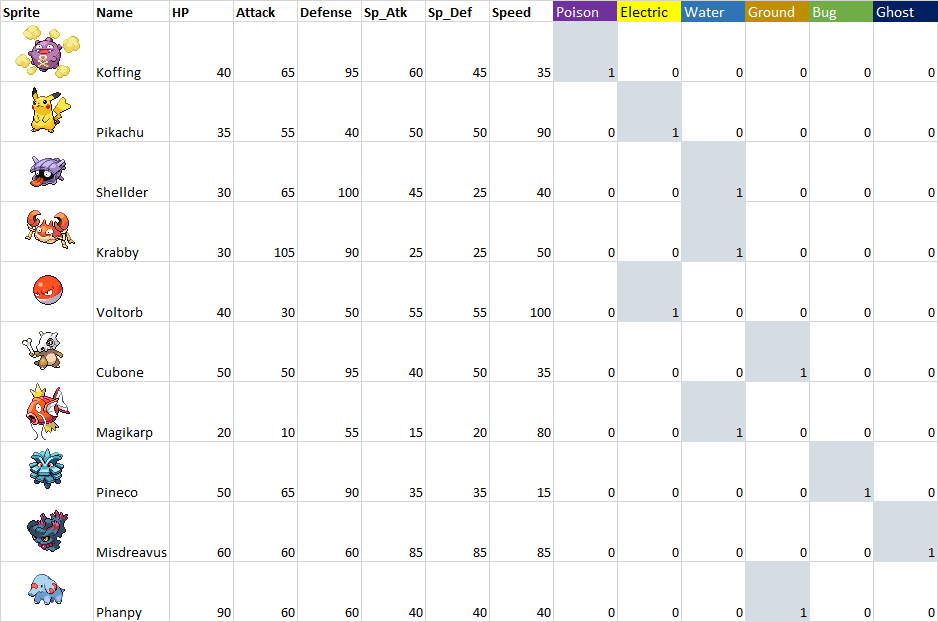
\includegraphics[width=1\linewidth]{figuras/pokemon1hot.png}
  \caption{One-hot encoding of Pokémon types.}
  \label{fig:pokehot}
\end{subfigure}
\caption{Table of a few Pokémon statistics representing its type as a \textbf{(a)} categorical variable or as an \textbf{(b)} one-hot encoding. In this case, the Pokémon types of a trainer could be represented by a bag-of-words by adding the one-hot encodings\footnote{Albeit it would be more of a ``bag-of-types'' than a bag-of-words}. Base stats from Generation VI from \citet{bulbapedia} and images from \citet{hotpokemon}.}
\label{fig:poke}
\end{figure}




However, these approaches are inefficient. Vocabularies tend to be huge, Merriam-Webster's Third New International Dictionary \citep{merriam} possesses $470,000$ different entries, but a typical sentence would not be longer than $100$ words. This leads to a sparse representation of sentences and also loses important information such as the order of appearance of the words in the sentence.

Embeddings are an efficient approach to solve these problems; an embedding is a low-dimensional space (in comparison to the huge size of typical vocabularies) into which one can translate high-dimensional vectors. In essence, an embedding tries to project into a lower dimensional space high-dimensional vectors in such a way that the ones that are ``similar'' are closer in the embedding space. In the case of words, we are interested in the semantic similarity between them but they may be similar in unexpected ways, depending on the training method antonyms may be closer than synonyms because they are used in similar ways.

Embeddings are not exclusive to natural language processing, they are used to deal with the sparsity of adjacency graphs, in graph neural networks, to permit the use of graphs as input for more conventional NNs \citep{grover2016node2vec} and may even be used with any machine learning model that deals with too many features, being particularly useful with boolean and categorical variables. They are also not exclusively used with individual words, they may be used with entire sentences \citep{sbert_paper}, paragraphs or even entire documents at once \citep{doc2vec}.


Another benefit of embeddings is that they have high re-usability, it is not uncommon to re-utilize them across different models and tasks. To further improve their performance there are many transfer learning techniques that can be leveraged, but depending on the application they may not even need fine tuning to achieve an acceptable performance.


We will now present an overview of an embedding called \textit{word2vec} to better illustrate embeddings and their uses.




\subsection{Word2vec}

Word2vec \citep{word2vec_original} is an algorithm that produces word embeddings. A word embedding as previously mentioned is a mapping of words into a vector space $\mathbb{R}^{n}$, i.e. each word can be represented as a vector of real numbers. 
The power of these embeddings created by word2vec comes from its dense distributed representation, wherein $\mathbb{R}^{n}$  is such that $n$ is smaller than the number of distinct words in the corpus and is capable of capturing some of the underlying syntactic and semantic structure of the language.

As an example of this structure we can take the vector representation for the words $king$, $queen$, $man$ and $woman$ and calculate  $king - man + woman$. This will provide us a new vector that is closer to $queen$ then any other word vector, as can be seen in the illustration of Fig.~\ref{queen}. In Figure~\ref{figur_word2vec} we can see other examples of such relationships captured by word2vec.





\begin{figure}[!ht]
\centerline{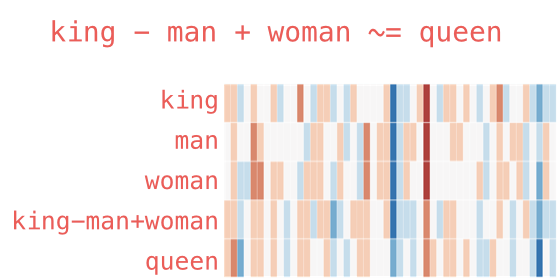
\includegraphics[width=0.8\textwidth]{figuras/queen.png}}
\caption{The resulting vector from ``king-man+woman'' doesn't exactly equal ``queen'', but ``queen'' is the closest word to it from the 400,000 word embeddings in this collection. Color coded cells based on their values (red if they’re close to 2, white if they’re close to 0, blue if they’re close to -2). \citep{jallamarword2vec}}
\label{queen}
\end{figure}




\begin{figure}[!ht]
\centerline{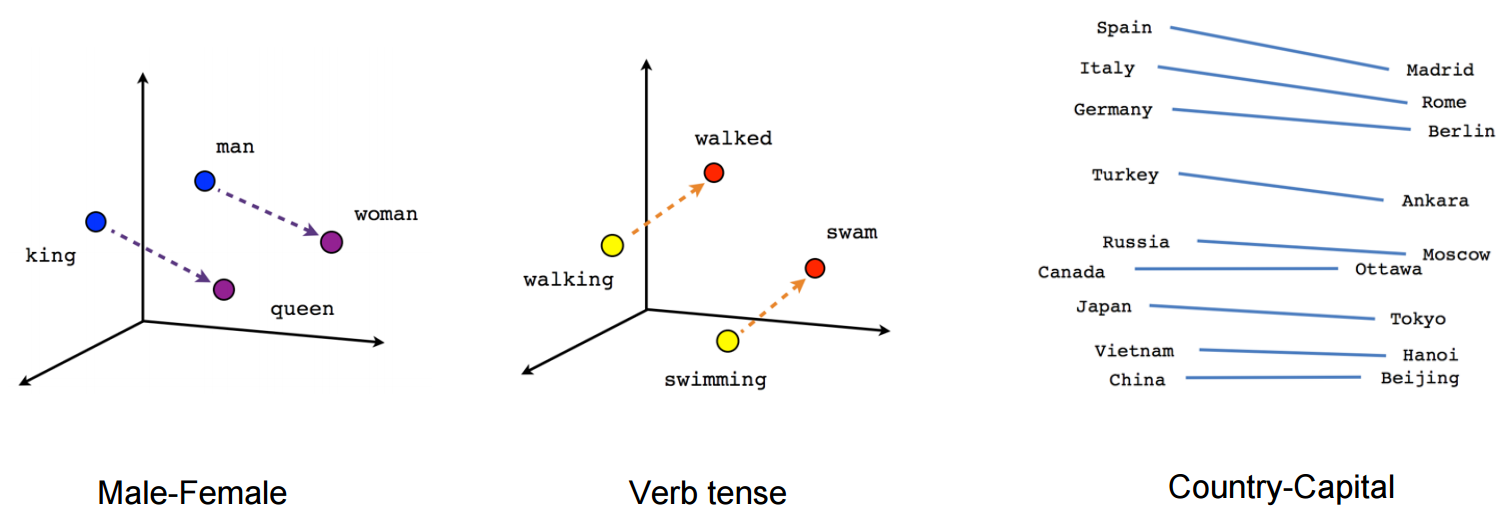
\includegraphics[scale=0.25]{ilustracao_word2vec}}
\caption{Illustration of some semantic and syntactic relations captured by word2vec embeddings, vectors whose words have similar relationships (such as gender or conjugation) tend to also have similar relations on the vector space \citep{ilustracao_word2vec}. This is nothing more than an illustration since usual embeddings are of such a high order that visualization as a simple 3D plot becomes impossible, dimensionality reduction techniques (e.g. PCA) albeit useful may lead to spurious relations, when searching for such relations it is customary to use appropriate distance metrics such as the cosine distance.}
\label{figur_word2vec}
\end{figure}

These relationships are obtained during its training process, at first each word is assigned a word embedding composed of purely random numbers that will converge into a meaningful embedding. The training process of this algorithm is based on the idea that one may deduce the meaning of a word by its context, so by updating the embedding of a word by using the embedding of its neighbors or vice-versa it is possible to capture semantic and syntactic information from the language thus construing a meaningful embedding space.

This idea of understating a word by its context is nothing new going at least as far as 1957:

\begin{myquote}
\textit{You shall know a word by the company it keeps.}\\
\citet{firth1957synopsis}
\end{myquote}

Word2vec was one of the first models to efficiently utilize this idea, being quickly followed by GloVe \citep{glove}, a model that leverages the co-ocurrence matrix of words to train its embedding, and many others. An example of a co-ocurrence matrix can be seen in Fig.~\ref{coocurence}. Even though nowadays there are many embeddings more powerful than those two, they are still useful for simpler applications as tried and tested methods or even because of their relatively high computational efficiency.


\begin{figure}[!ht]
\centerline{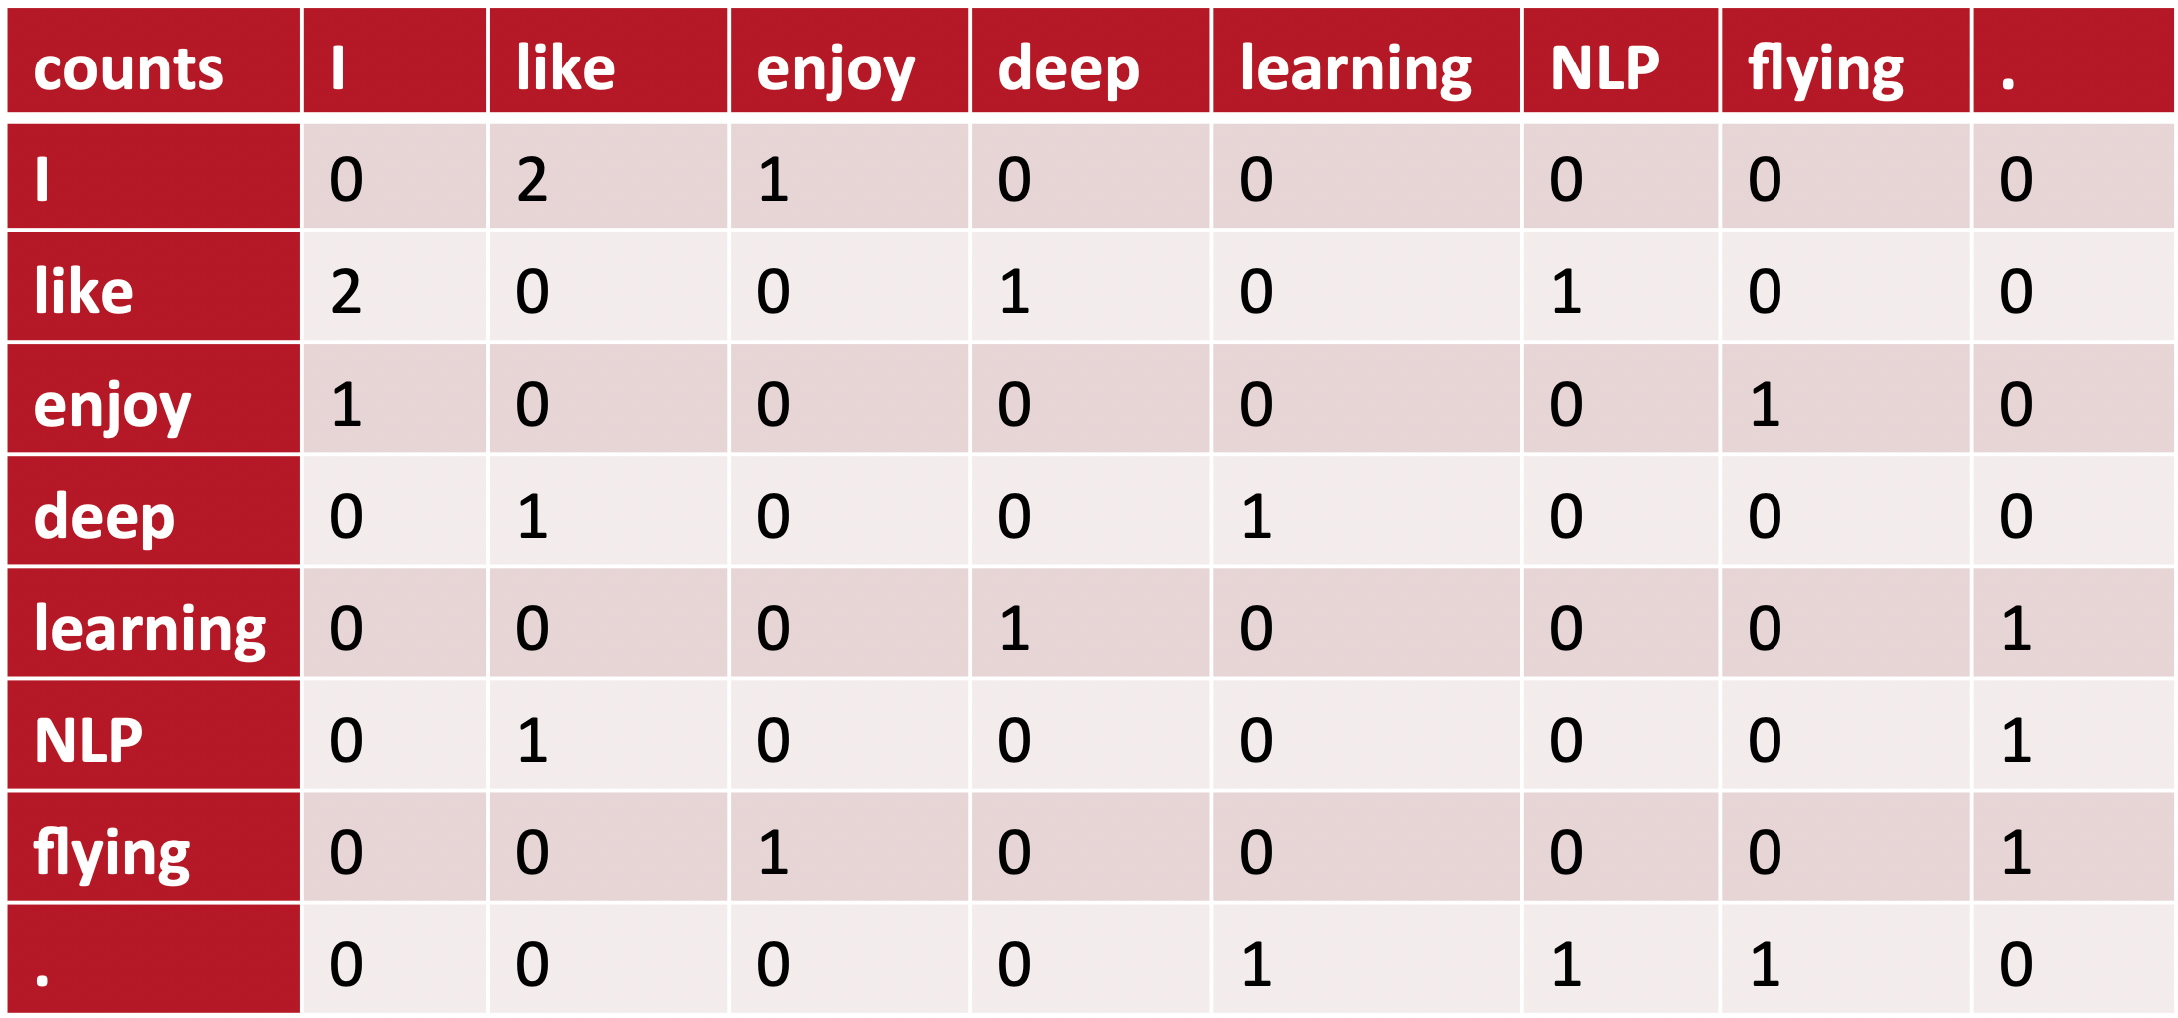
\includegraphics[width=0.85\textwidth]{figuras/coocurence.png}}
\caption{Example of a co-ocurrence matrix with a symmetrical window of size 1.\\
Corpus: I like deep learning. I like NLP. I enjoy flying.\\
Dictionary: [ 'I', 'like', 'enjoy', 'deep', 'learning', 'NLP', 'flying', '.' ] \citep{coocurrence}
}
\label{coocurence}
\end{figure}

\section{LSTM}

\begin{figure}[!ht]
\centerline{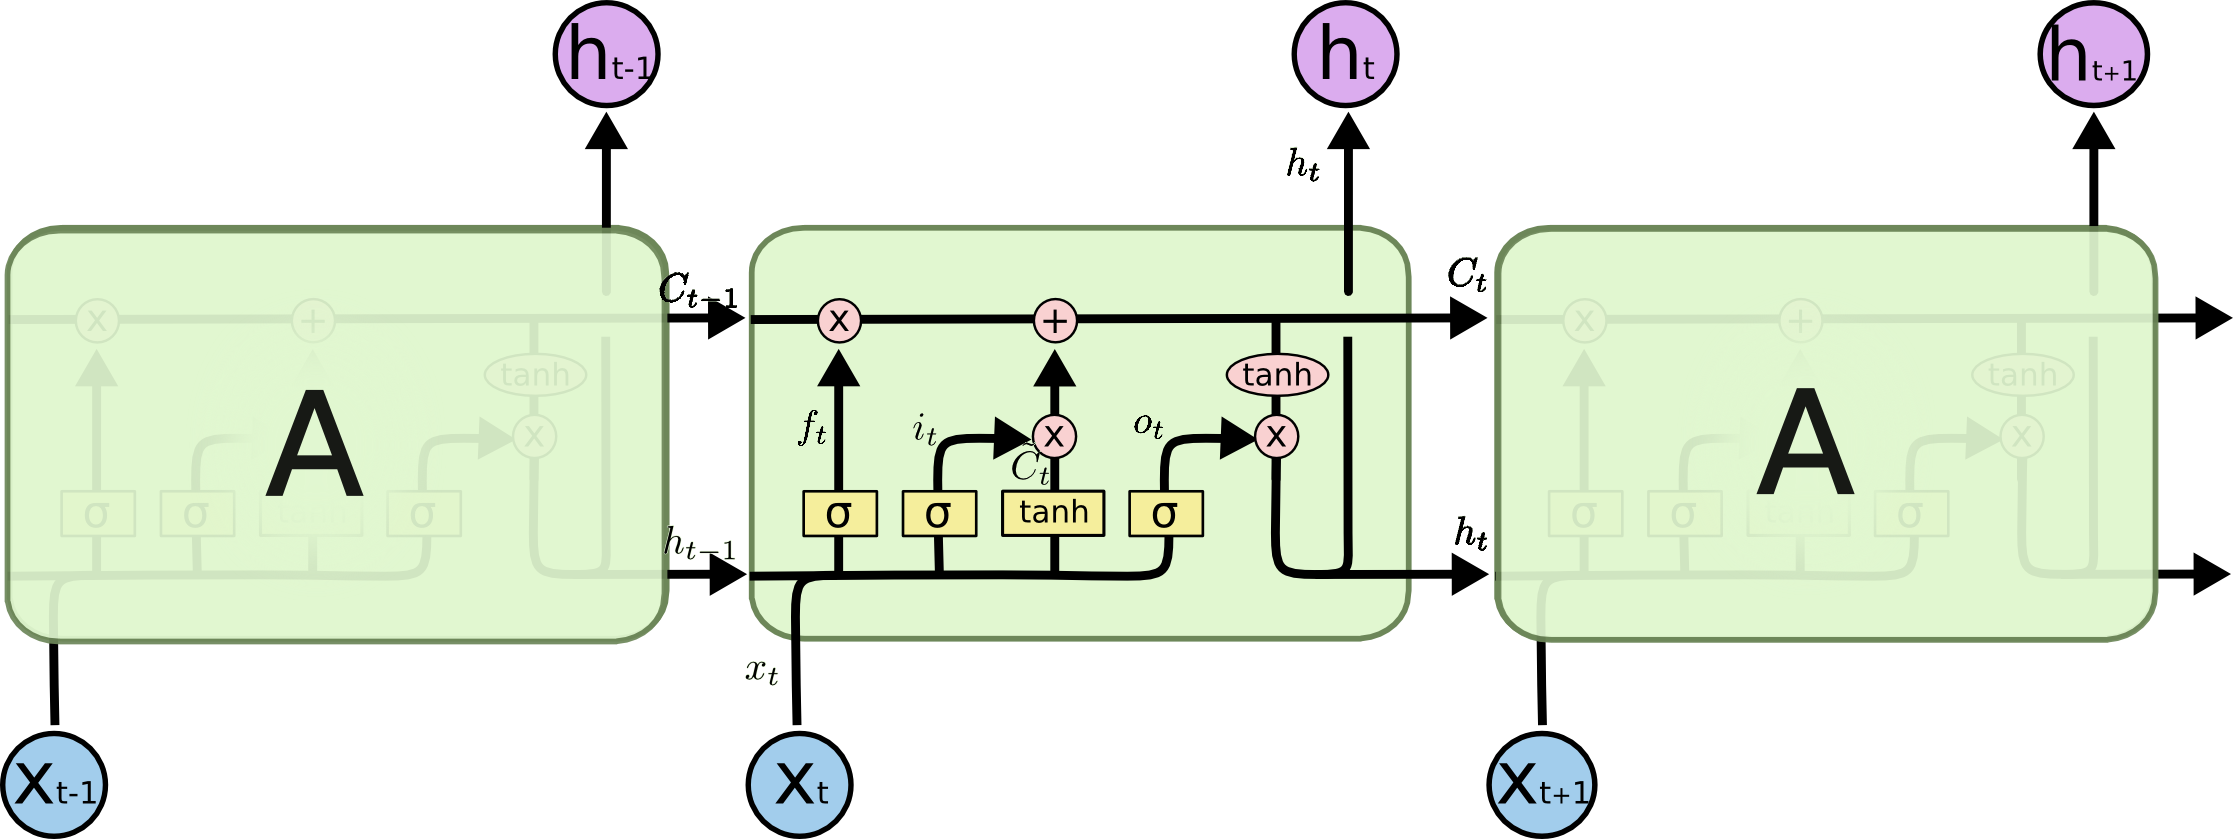
\includegraphics[width=1.1\textwidth]{figuras/lstm.png}}
\caption{An illustration of the LSTM architecture, image adapted from \citet{lstm_imagem}.
}
\label{fig:lstm}
\end{figure}

LSTM, or Long Short-Term Memory \citep{lstm}, is a recurrent neural network architecture developed to tackle the problem of vanishing gradient when dealing with long inputs in RNNs where the ``gradient flow'' would vanish, resulting in stagnation during training and the inability to deal with long distance relationships in, for example, long sentences or paragraphs. This inability to go beyond ``short-term memory'', was improved by introducing a better information flow in the network, giving it the ability to learn when to ``forget'' and when to ``update'' accordingly.
An illustration of this architecture can be seen in Fig.~\ref{fig:lstm}, but it can be described by its three gates:

\begin{itemize}
    \item[] Forget gate:  $f_t = \sigma(W_f . [h_{t-1},x_t] + b_f)$
    \item[] Input gate: $i_t = \sigma(W_i . [h_{t-1},x_t] + b_i)$
    \item[] Output gate: $o_t = \sigma(W_o . [h_{t-1},x_t] + b_o)$ 
\end{itemize}

The forget gate is responsible for ``deciding'' what to keep from earlier steps, the input gate for what to keep from the current step and the output gate for the next hidden state $h_t$. Another integral part of this model is the cell state $C_t$ and the \textit{candidate} cell state $\tilde{C}_t$, responsible for ``storing'' the information on the network, being updated at each time step based on the candidate cell state, the input gate and the forget gate:


\begin{itemize}
    \item[] $\tilde{C}_t = \textit{tanh}(W_C . [h_{t-1}, x_t] + b_C)$
    \item[] $C_t = f_t * C_{t-1} + i_t * \tilde{C}_t$ 
    \item[] $h_t = o_t * \textit{tanh}(C_t)$
\end{itemize}


\section{Encoder-Decoder}
The idea behind the encoder-decoder neural network architecture is to use an encoding layer to create an intermediary representation of the input that will subsequently be transformed by the decoder layer into the desired target.
Recurrent neural networks such as LSTMs or GRUs \citep{GRU} are commonly used as the encoding and decoding layers to avoid the vanishing gradient problem. %, they are able to do so by using feedback loops to obtain information persistency.
 A common use of the encoder-decoder architecture is machine translation through seq2seq \citep{seq2seq}. For example, an english text can be used as an input to the encoder which will generate a latent space vector, an abstract representation of the text, that will be used by the decoder to generate a french translation of the original text. This process can be visualized in Fig.~\ref{contextvec}.

\begin{figure}[!ht]
\centering
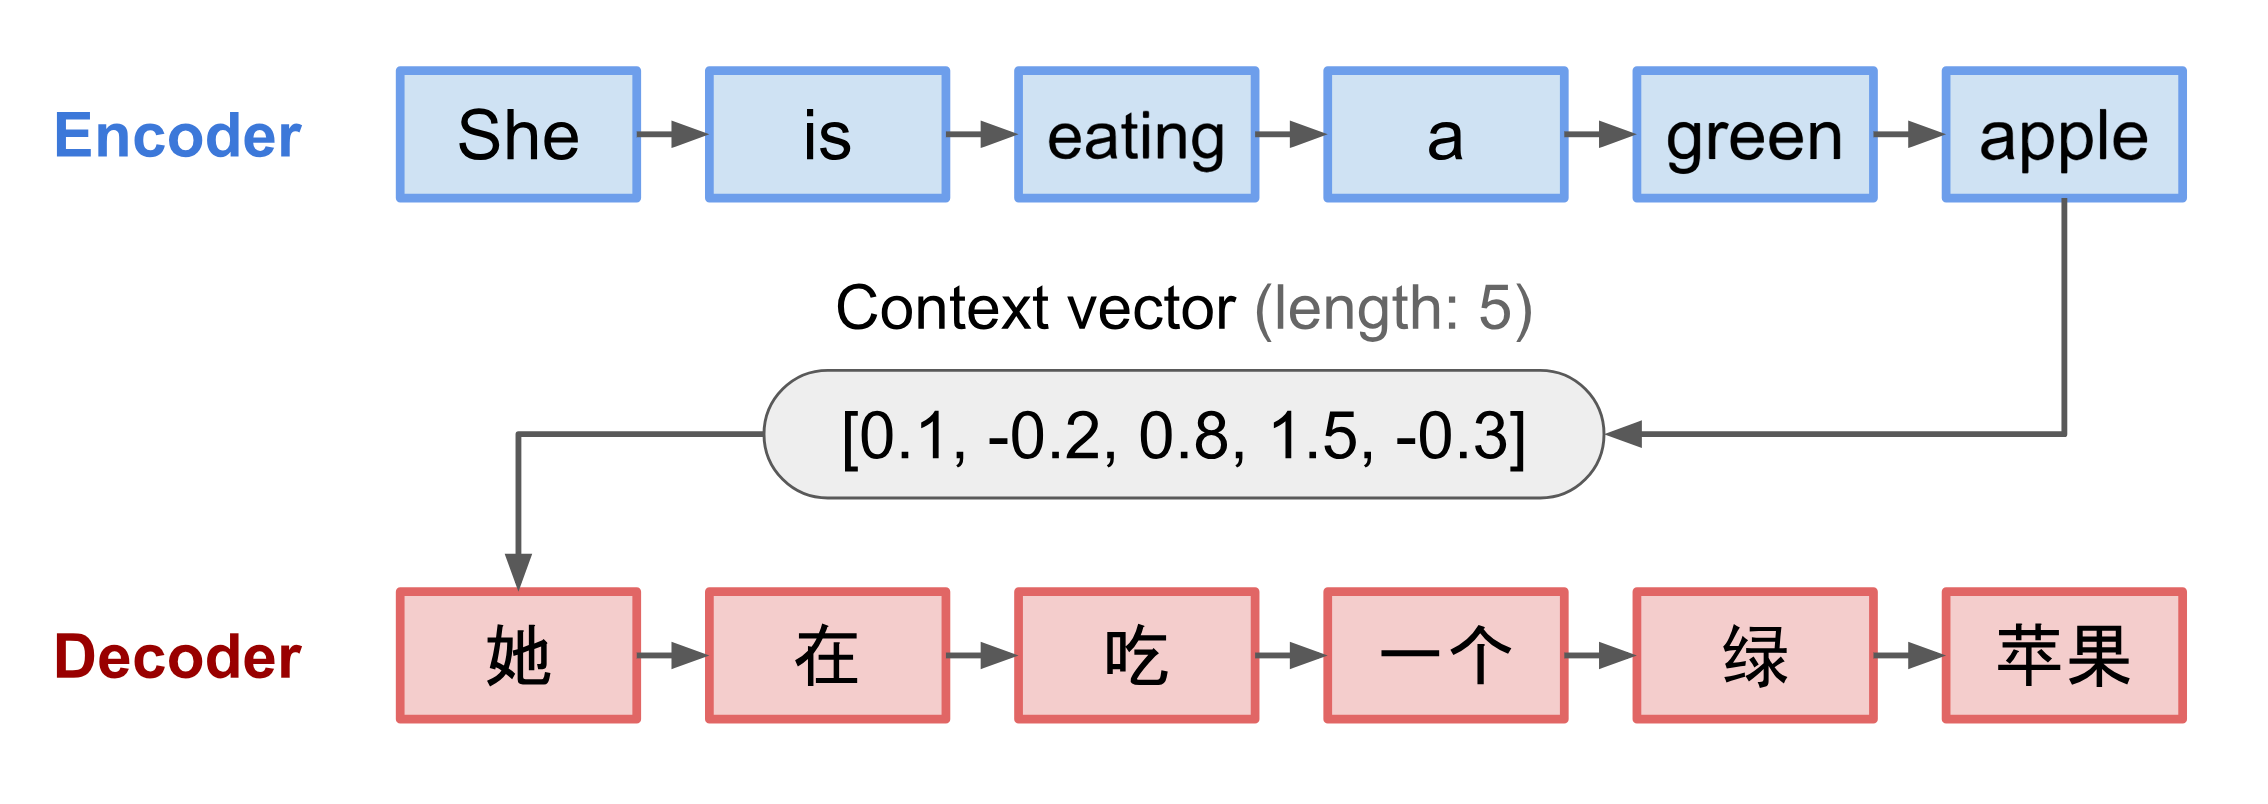
\includegraphics[width=0.9\textwidth]{figuras/context_vector.png}
\caption{\textit{The encoder-decoder model, translating the sentence ``she is eating a green apple'' to Chinese. The visualization of both encoder and decoder is unrolled in time.} \citep{weng2018attention}\\ The context vector in gray is the intermediary representation between the encoder and decoder that needs to hold all the relevant information to successfully realize the translation without referencing the original input in english. }
\label{contextvec}
\end{figure}


Another example of the encoder-decoder architecture are the autoencoders, where the objective is to make the output predict the input. The existence of an intermediate state outputted by the encoder forces the autoencoder to learn a compact representation of the input and try to reconstruct it as the output, an illustration can be seen in Fig.~\ref{autoencoder}.


\begin{figure}[!ht]
\centering
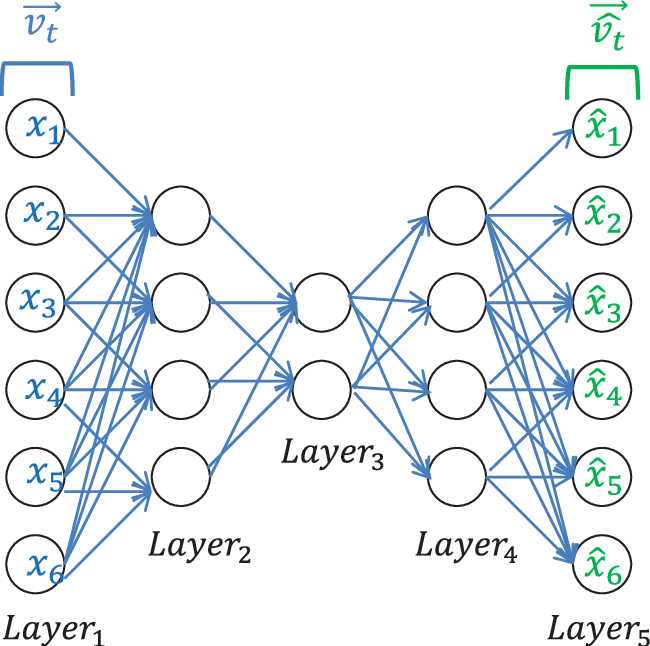
\includegraphics[scale=0.3]{An-illustration-of-AE-learner.png}
\caption{Illustration \citep{imagem_autoencoder} of a shallow autoencoder. $\vec{v}$ and $\vec{\hat{v}}$ represent the input and output respectively of the network while the output from layer 3 is responsible for the compact representation of the input on the latent space. The encoder is composed of layers 1, 2 and 3 while the decoder is composed of layers 4 and 5.}
\label{autoencoder}
\end{figure}

\section{Attention}
Attention comes to address one of the main drawbacks of the encoder-decoder architectures, the informational bottleneck. By forcing the entire sequence of information to be contained in a single vector it becomes increasingly difficult to capture long-range relations and information presented at the beginning of long input sentences. 
Attention provides a simple manner of capturing the relevant input tokens for each token of the output, generating an attention matrix that represents the relevant context for each token and improving interpretability.


\begin{figure}[!ht]
\centerline{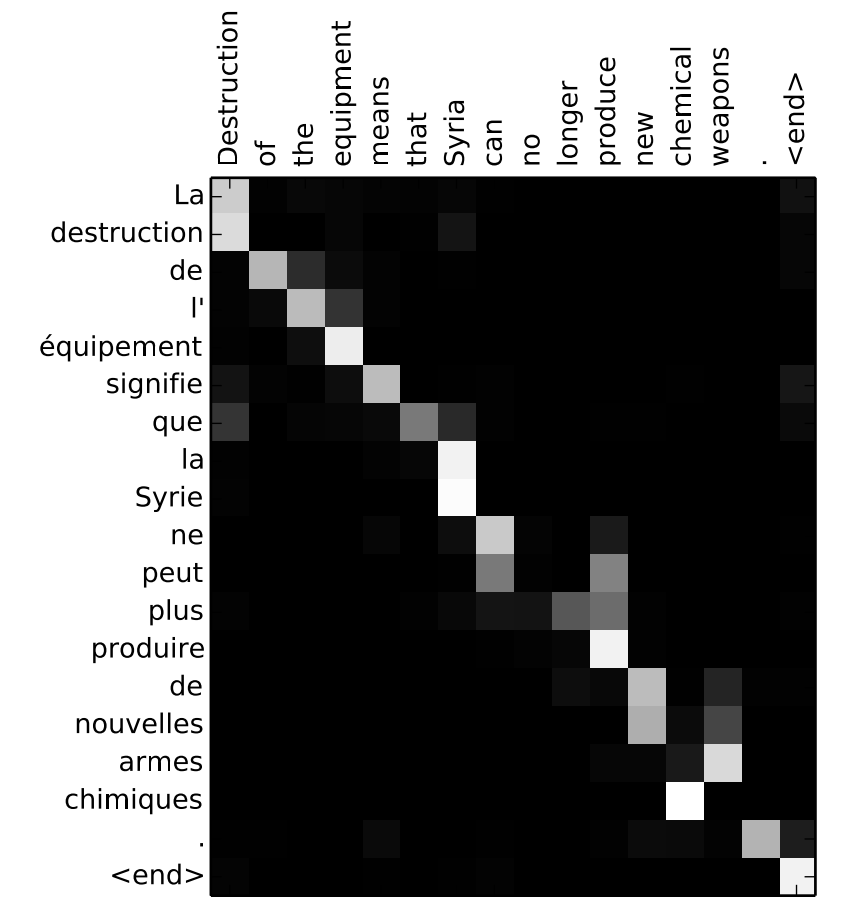
\includegraphics[scale=0.5]{attention_matrix.png}}
\caption{Illustration \citep{attention_matrix} of an example attention matrix for a sentence in english and it's french translation. }
\end{figure}

This provides another counter-measure against the vanishing gradient problem by connecting the entirety of the input to the training process, but the biggest insight of attention is this idea of paying attention to a specific part of the input that is more relevant to obtain our desired output. For example, given the obscured photo in Fig.~\ref{img:dog_escondido} how would one describe its content? We could guess about the gender, origins or facial expression of the depicted person, but we would most likely assume it depicts a human and not a dog as can be seen in Fig.~\ref{img:dog}, but how did we arrive at this conclusion? Which part of the image implies the presence of a human? This is the essence of the idea behind attention, where to look at to answer something. 





\begin{figure}
\centering
\begin{subfigure}{.45\textwidth}
  \centering
  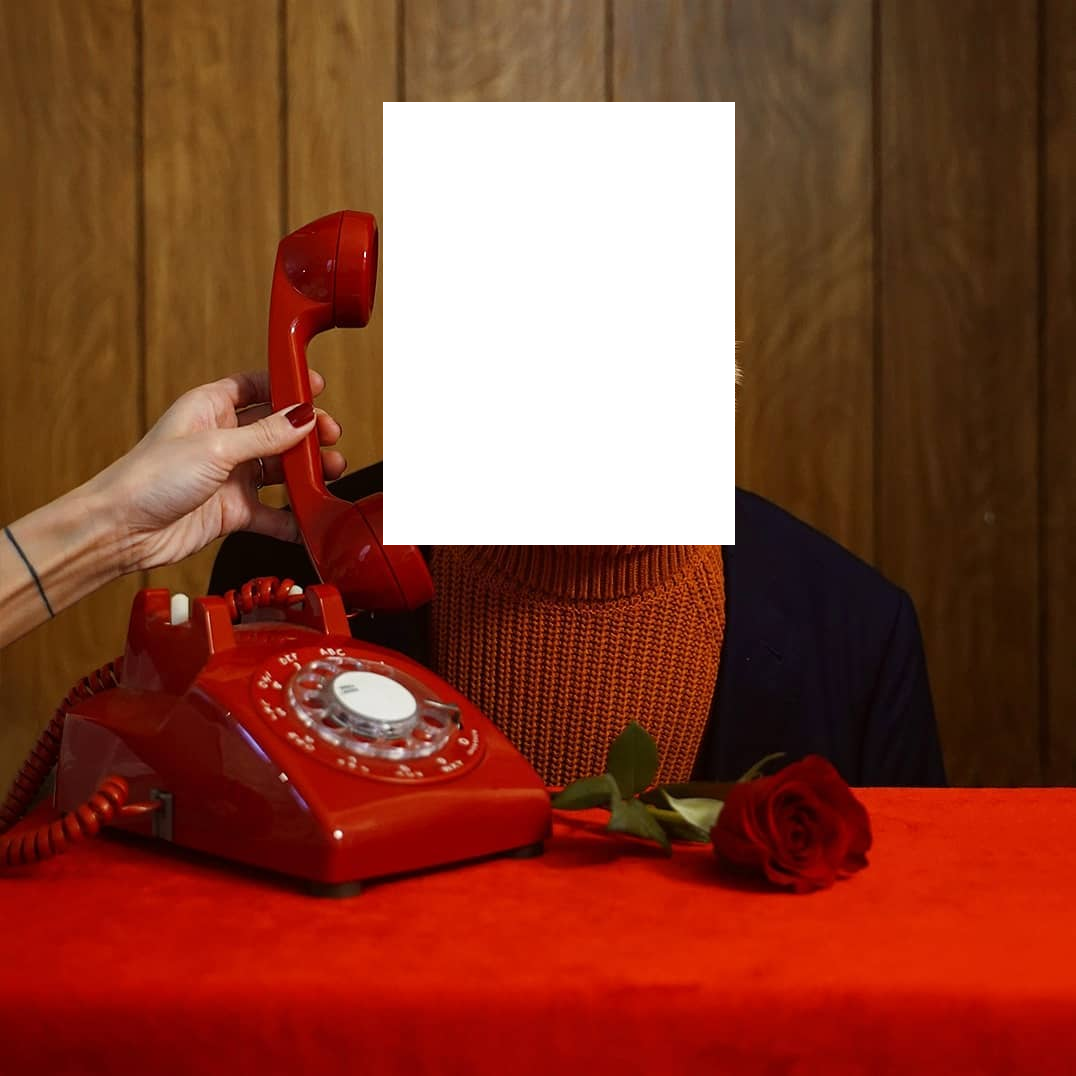
\includegraphics[width=1\linewidth]{figuras/dog_obscuro.png}
  \caption{}
  \label{img:dog_escondido}
\end{subfigure}
\begin{subfigure}{.45\textwidth}
  \centering
  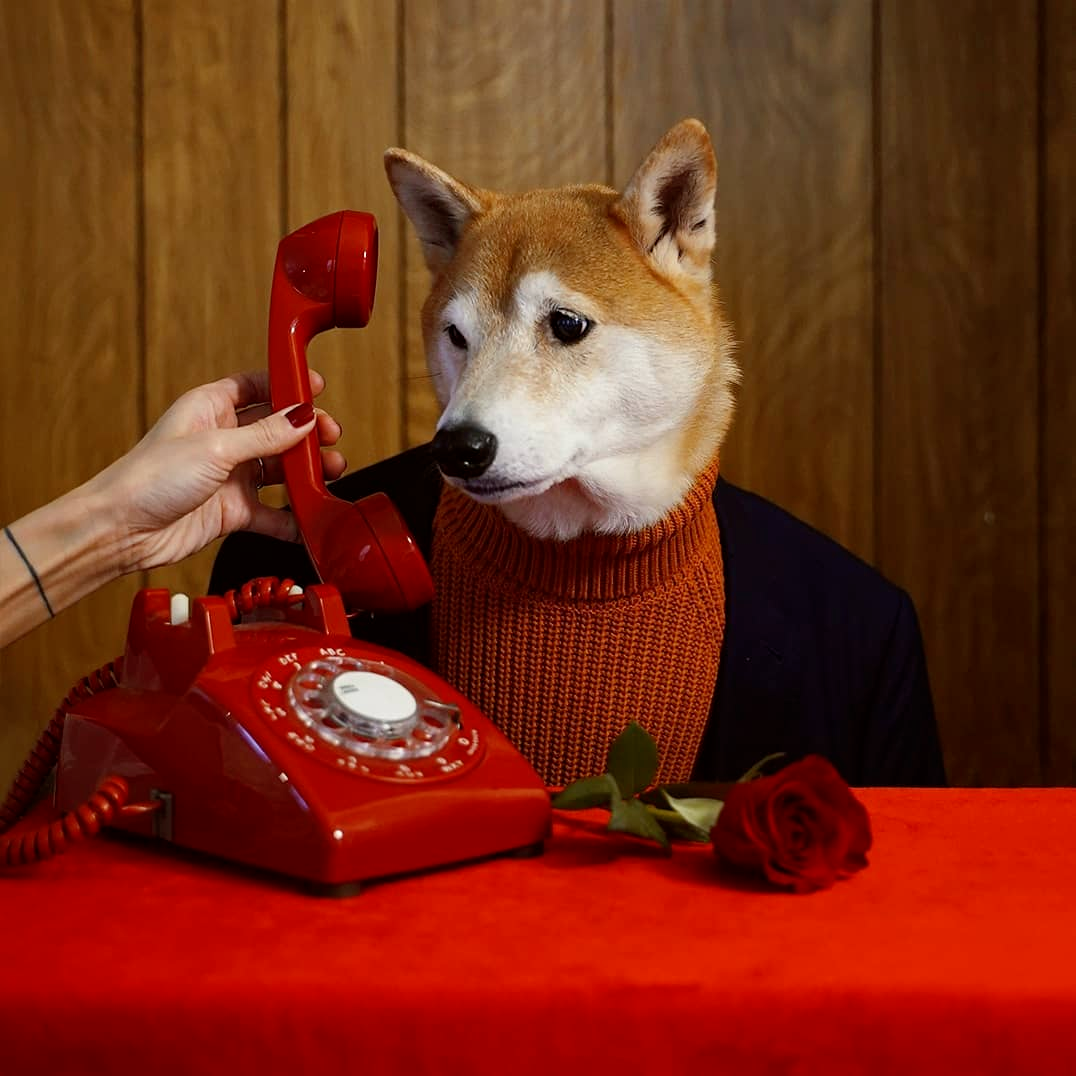
\includegraphics[width=1\linewidth]{figuras/dog.png}
  \caption{}
  \label{img:dog}
\end{subfigure}
\caption{A collage to illustrate the idea of attention and visual attention. Photo obtained from \citet{dog}.}
\end{figure}



\citet{atencao_review} generalized attention by breaking it into three swappable components: the 3-tuple (key, query, value), the score function and the distribution function. 
% Since many new types of attention were being continuously developed, a framework to generalize them was, and still is, necessary to better understand and differentiate them. If this particular nomenclature will take root on the machine learning community or not only time can tell, but we will be adopting it in this work nevertheless.


The tuple (key, query, value) are the input for the score function, the objects upon which we desire to calculate the attention. The score function is used to calculate the energy scores that will be subsequently passed through the distribution function to produce the attention scores such as the \textit{softmax} function that also normalizes the scores into a probability distribution.

Fig.~\ref{fig:atencao_geral} illustrates this general framework and Fig.~\ref{img:luong} gives an illustrative example of one of the first attention implementations.

  
\begin{figure}[!ht]
\centering
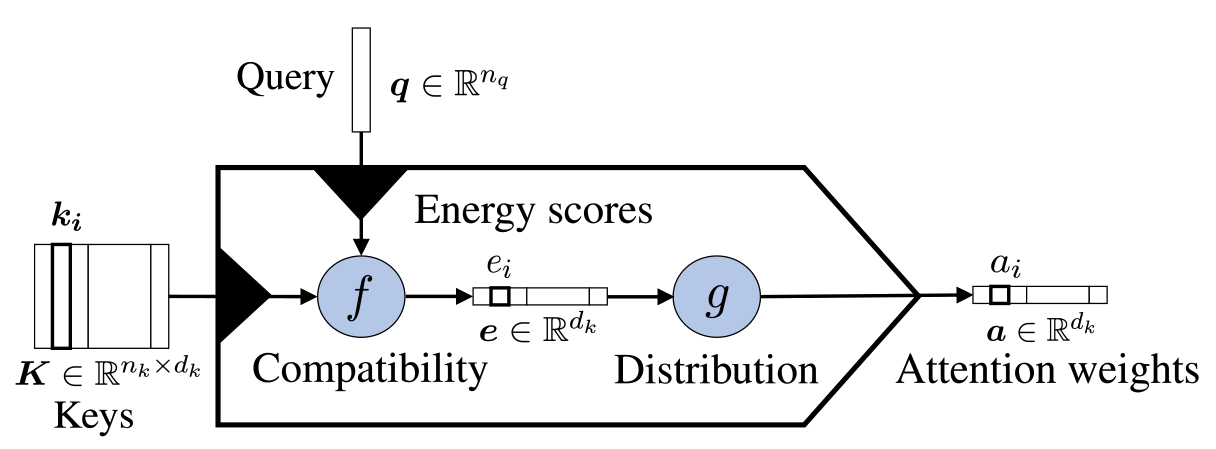
\includegraphics[width=0.8\linewidth]{figuras/atencao_geral.png}
\caption{Illustration of \citet{atencao_review} general attention framework. The ``Value'' component is not present in this illustration but could be used in a subsequent step to process the attention scores to create a context vector. }
\label{fig:atencao_geral}
\end{figure}


\begin{figure}
\centering
\begin{subfigure}{.5\textwidth}
  \centering
  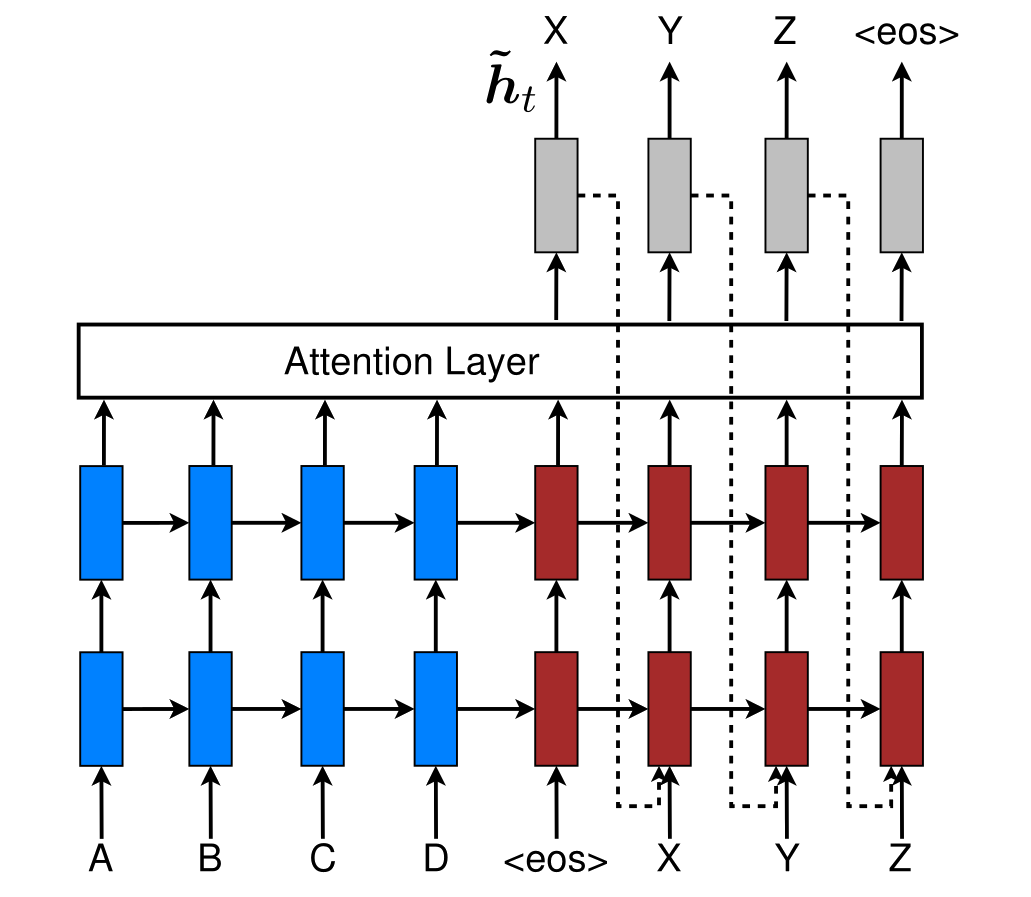
\includegraphics[width=1\linewidth]{figuras/luong1.png}
  \caption{Illustration of an encoder decoder model with attention, every decoder step decides the next token based on the context vector and the last decoder hidden state. The blue rectangles represent the encoder and the red ones the decoder.}
  \label{img:luong1}
\end{subfigure}
\begin{subfigure}{.75\textwidth}
  \centering
  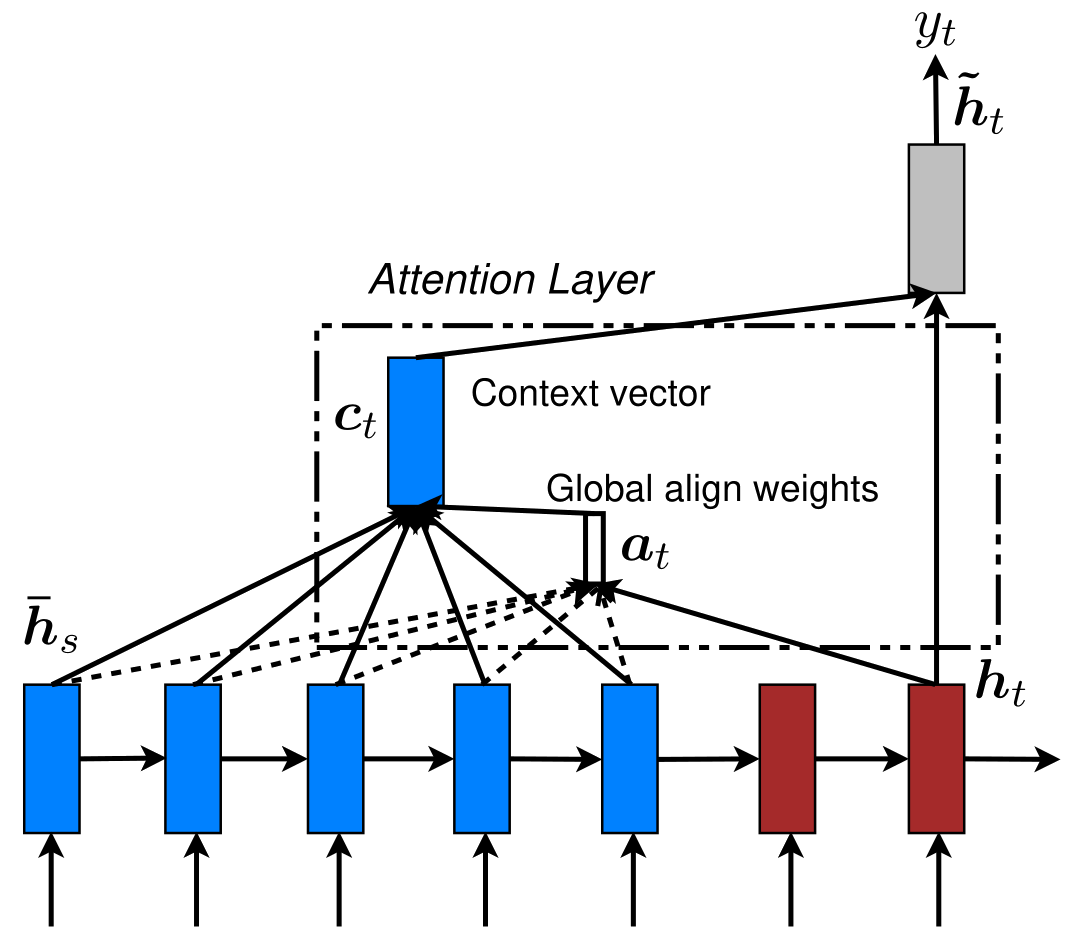
\includegraphics[width=1\linewidth]{figuras/luong2.png}
  \caption{To calculate the attention all encoder hidden states $\bar{h_s}$ (Keys)\footnote{In this case Key and Value are the same} and the current decoder hidden state $h_t$ (Query) are passed to the score function $score(h_t, \bar{h}_s) = h_t^\top \bar{h}_s$ to calculate the energy scores. Then the energy scores are passed to the distribution function softmax $a_t(s)= \frac{exp(score(h_t, \bar{h}_{s}))}{\sum_{{{s}}'} exp(score(h_t, \bar{h}_{{s}'}))}$ to generate the attention score.
    How to use an attention score may vary between architectures and applications, in this particular case \citet{luong2015effective} takes the weighted average $c_t =\frac{\sum_s \bar{h}_i a_i}{|s|}$ of all attention scores to create a context vector which will be used with the decoder hidden state to predict the next word.
}
  \label{img:luong2}
\end{subfigure}
\caption{Fig.~\ref{img:luong1} illustrates an encoder decoder model and Fig.~\ref{img:luong2} illustrate its attention mechanism, both images extracted from \citet{luong2015effective}.}
  \label{img:luong}

\end{figure}






\section{Pointer Networks}
\label{sec:ptrnet}
Pointer Net \citep{pointer}, or Ptr-Net, is a neural architecture that learns the conditional probability of an output sequence composed of index positions of the input sequence. It is essentially an encoder-decoder architecture with attention, but the attention mechanism is used at each step to determine an index of the input. Fig~\ref{ptr_hull} illustrates the difference from a normal encoder-decoder.


\begin{figure}[!ht]
\centering
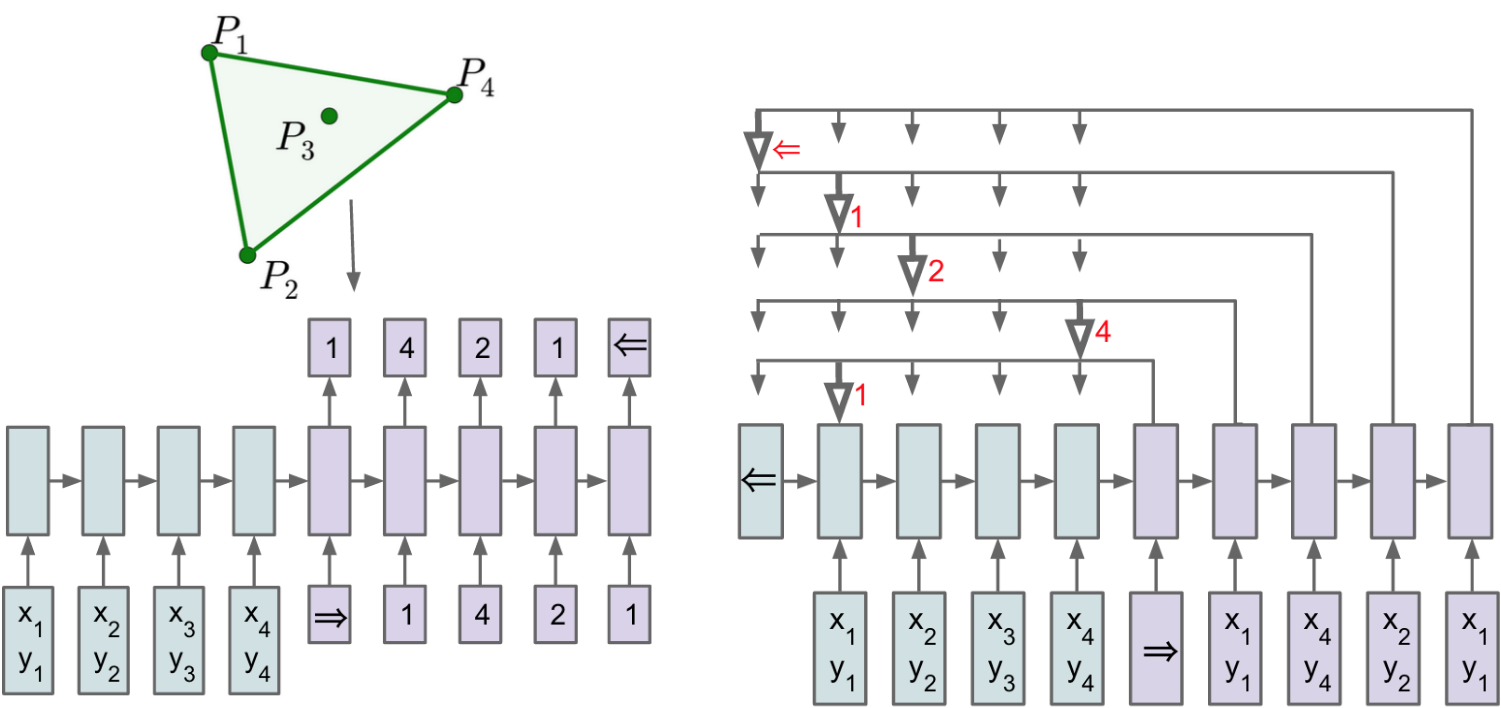
\includegraphics[scale=1.2]{figuras/ptrjunto.png}
\caption{This illustration represents 2 different architectures used to find the convex hull of a set of points \citep{pointer}. The left one is a normal encoder-decoder while on the right we have a Ptr-Net. } 
\label{ptr_hull}
\end{figure}

The original paper explores the use of this architecture with geometric problems, such as finding the convex hull as can be seen in Fig~\ref{ptr_hull}, but it can also be used for other problems. Another use of Ptr-Nets are in Q\&A tasks such as in the SQuAD dataset \citep{squad1} where a question is provided paired with a text that contains the answer to this question. A common approach \citep{squad_pointer} to answer the question is to train a model that finds in the provided text an initial and a final token that together delimit a minimal portion of the text that contains the answer. An example of such a Q\&A task can be seen on Fig.~\ref{squad}.

  
\begin{figure}[!ht]
\centering
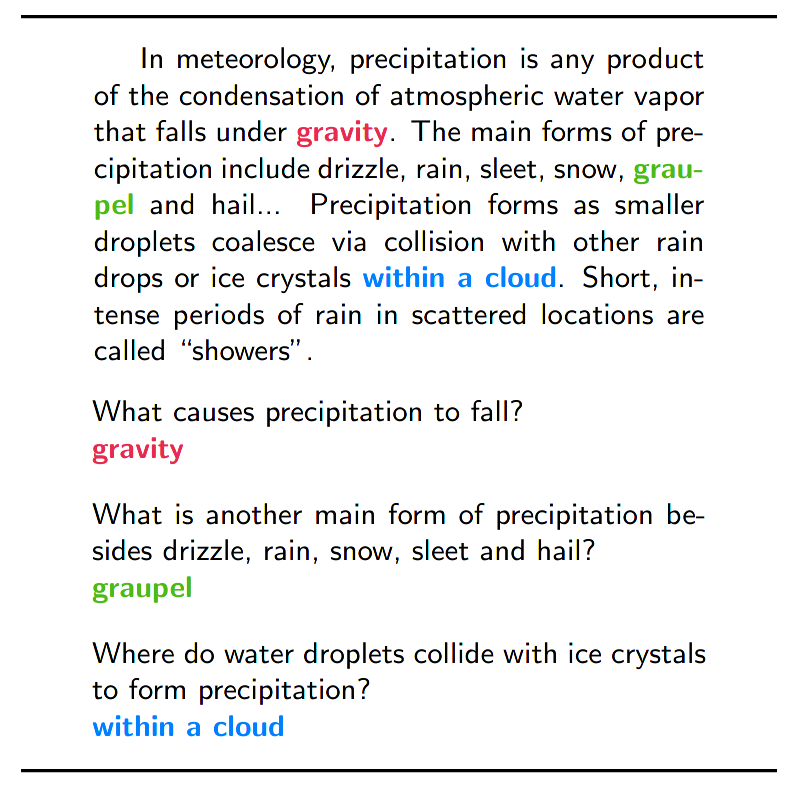
\includegraphics[scale=0.3]{squad.png}
\caption{This excerpt illustrates 3 different questions for a single paragraph of text, for the first two questions the initial and final tokens overlap as the answer is composed of a single word. On the third question the initial token would be the word ``within'' and the final token would be ``cloud'' and the resulting answer delimited by them would be ``within a cloud''. Example extracted from \citep{squad1}.}
\label{squad}
\end{figure}




\section{Transformer}
The transformer \citep{attention_is_all_you_need} is another encoder-decoder architecture but with a major difference: it shifts from the use of recurrent neural networks in favor of attention. More precisely, the encoder uses word vectors as input and is composed of a self-attention layer followed by a feed forward network.
Self-attention is capable of capturing strong semantic information, for example in the sentence ``Marie bought a cookie and ate it.'' the self-attention model is capable of determining that the token ``it'' refers to the token ``cookie''.


The transformer starts by using self-attention on the word embeddings to aggregate information from each token, creating a new context-rich representation for each word simultaneously. The decoder on the other hand takes an iterative approach, instead of outputting the entire translated sentence at the same time it generates one word at a time. The decoder utilizes the final representation output by the encoder and every word it already output to generate the next word until it predicts and $<END>$ tag. In essence it will receive the sentence to be translated as input and will output the translated sentence one word at a time. Figs.~\ref{trans_arq} and \ref{self-att} illustrate the architecture of the transformer model and the self attention mechanism.

\begin{figure}[!ht]
\centering
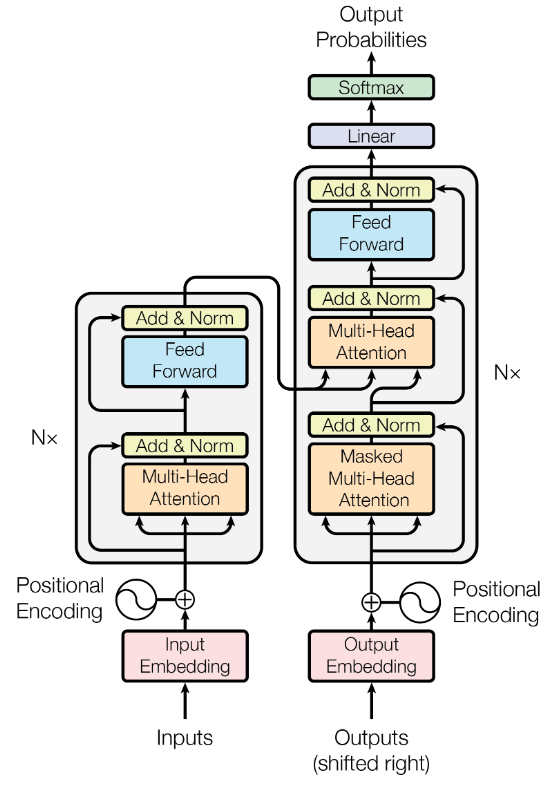
\includegraphics[scale=0.6]{figuras/transformer_arquitetura.png}
\caption{The Transformer - model architecture. \citep{attention_is_all_you_need}}
\label{trans_arq}
\end{figure}


\begin{figure}[!ht]
\centering
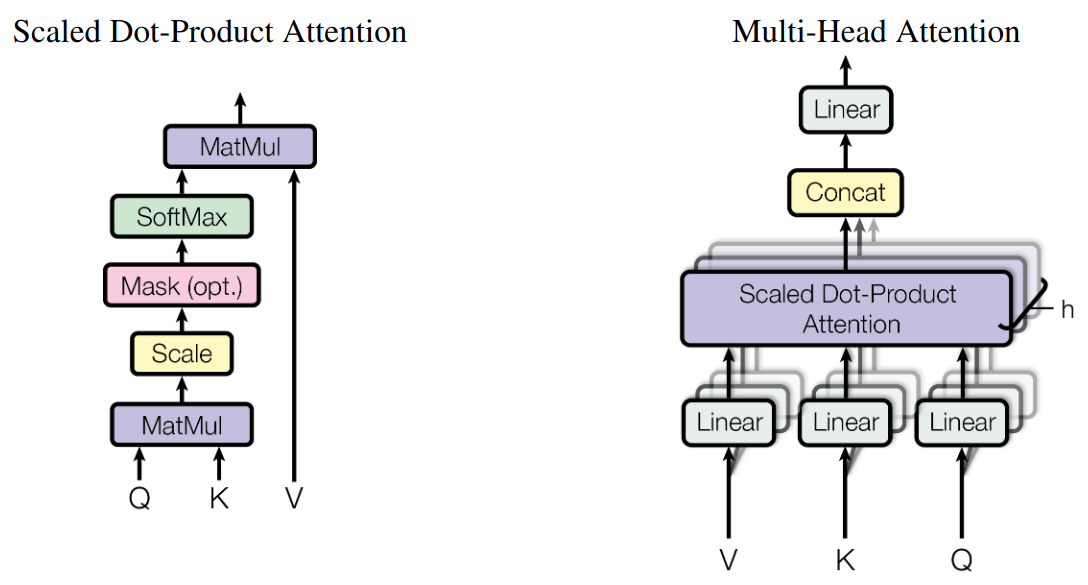
\includegraphics[width=0.9\textwidth]{figuras/self-att.png}
\caption{(left) Scaled Dot-Product Attention. (right) Multi-Head Attention consists of several
attention layers running in parallel. \citep{attention_is_all_you_need}}
\label{self-att}
\end{figure}

The transformer architecture achieved state of the art performance in translation tasks and, due to its focus in attention, it was able to be trained significantly faster than other models centered around recurrent or convolutional layers. This led to a series of new models based on the transformer architecture and the idea that attention is all you need,  one of its variants, a masked-language model composed of stacked Transformer encoders called BERT \citep{BERT}, quickly became the new baseline for NLP tasks such as \citep{rogers-etal-2020-primer}, including classification tasks.

The BERT model is capable of considering the context of a word occurrence, differently than the previously mentioned context-free embeddings word2vec an GloVe. For example, the vector for ``running'' would have different embeddings in BERT for the phrases ``He is running the company into the ground.'' and ``He is running away'' while word2vec would produce the exact same embedding.




\section{Typical seq2seq Metrics}
~\label{sec:bleu}


BLEU \citep{bleu}, or \underline{b}i\underline{l}ingual \underline{e}valuation \underline{u}nderstudy, is a corpus wide NLP metric frequently used for sequence to sequence tasks such as machine translation or text summarization. This metric is a normalized score for \textit{n}-grams overlap between the output and reference outputs (e.g. reference translations in a machine translation task) with a brevity penalty for shorter outputs.

Despite BLEU's wide spread use, it has some flaws. Among the main problems pointed out by the community are the metric's inability to take meaning and sentence structure into account, e.g. a rarer synonym could penalize a correct translation and a random shuffle of words of a correct translation could have a similar BLEU score albeit being complete nonsense \citep{bleu_shuffle}.


Another famous benchmark is the previously mentioned SQuAD 1.X \citep{squad1} and its successor SQuAD 2.0 \citep{squad2}, these are reading comprehension datasets that consist of questions posed by crowdworkers on a set of Wikipedia articles. The answers may or may not be contained in the corresponding reading passage upon which the question is theoretically posed, SQuAD 2.0 being composed of the questions from SQuAD 1.1 and 50,000 unanswerable ones written to look similar to answerable questions.
